
\section{Evaluation}\label{sec:eval}

In order to test the efficiency of Dynamic Delay Scheduling, we have designed several 
tests, on both a small and a large scale, using our implementation in Spark, with fair
scheduling enabled. The goal of
these experiments is to demonstrate that an adaptive delay interval provides decreased
job latency in a variety of cluster setups and workloads.

\subsection{Evaluation Setup}
Our small-scale tests were performed on a four node local cluster, with four
task slots (four 1.6 GHz cores for Spark tasks) per machine. All four nodes were
connected through a Gigabit Ethernet switch. The workload chosen for the
small-scale test was an integer sort, on 1GB of input data spread across HDFS.
The main goal behind the small-scale setup is to evaluate our algorithm in a
controlled environment with stable network conditions. To provide data locality
concerns, input data was placed on two nodes, so as to ensure both data-local
and non-local slots for task placement.

In order to have a more realistic evaluation, our large-scale tests were
performed on a 16 node cluster on Amazon EC2, using m3.xlarge instances. The
workload chosen for the large scale test was a TPC-H benchmark, which
performs queries reading from multiple databases in HDFS, of size ranging from
several megabytes to 80 gigabytes (for a total of ~110GB of input data).
We chose this particular benchmark because each query
consists of a mixture of large and small stages which read from and process these tables
in parallel. This causes contention for resources in the cluster, creating
situations in which locality and fairness clash. This benchmark also represents
a workload in which fairness is likely to be desired. Without fair sharing,
stages which read from small tables would be significantly delayed by
longer-running stages operating on larger data sets. Queries 11, 12, and 22 failed
to terminate in any configuration (perhaps due to bugs in the query implementation),
and have been omitted from the figure.
All numbers, from both small and large scale, are the average of 3 runs.

\subsection{Small Scale Results}
%\masoud{@Derek: Argue why sort is a good application for our controlled small
%scale eval} 
The results of our small-scale tests are shown in Figure~\ref{fig:smallscale}.
We chose sorting for this test because sorting is an IO-bound job, meaning that
the effects of delay scheduling (increasing data locality) are more important
to overall job performance.
We performed the sort first with no delay at all, then with the default fixed 3 second delay,
and then with dynamic delay scheduling enabled. The default of
3 seconds causes a slight increase in completion time (versus no delay). Given
that network conditions were very good between the nodes in the cluster (all were
connected to the same switch), having a fixed delay value of 3 seconds causes
increased overhead, because the network overhead of missing locality is far
shorter than 3 seconds. Our adaptive solution performs slightly better, because
the delay interval shrinks based on the feedback from the first round of tasks,
although the job is still too small for there to be the kind of resource
contention that would result in larger speedups. This experiment simply
demonstrates that an incorrect fixed delay interval can actually hurt the
performance of a job, rather than improve it.

\subsection{Large Scale Results}

The results of our large-scale TPC-H tests are shown in Figure~\ref{fig:largescale}, with the same three 
delay setups (no delay, fixed 3 seconds, and dynamic). In every query tested, Dynamic Delay
Scheduling had lower job latency than the default fixed delay, by roughly 10\% per query. With
these being large workloads with hundreds of tasks, there is a great deal of contention for
slots amongst all running stages, creating both more accurate feedback over time and
more opportunities for delay scheduling to benefit job latency. The benefit is largest
in the longer queries, where there are both large and small stages competing for slots.
In the shorter queries, we can see that a dynamic delay at least does not add any overhead,
as the default delay does in queries Q2, Q13, and Q16. This shows that Dynamic Delay Scheduling
can lower job latency by both a) removing excess waiting time in small jobs, and by b) 
improving fairness vs. performance decisions in jobs with high resource contention.

\begin{figure}[t]
    \minipage{0.5\textwidth}
        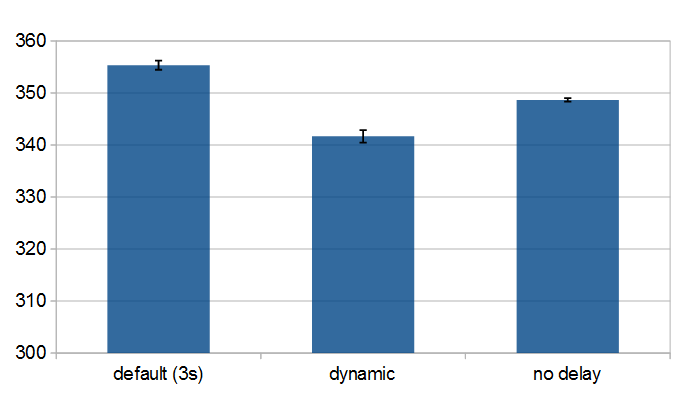
\includegraphics[width=\linewidth]{./smallscale.png}
        \caption{1GB Spark Sort - Job Completion Time (s) vs. Delay Type}
        \label{fig:smallscale}
    \endminipage \hfill
\end{figure}

\begin{figure*}[t]
    \minipage{\textwidth}
        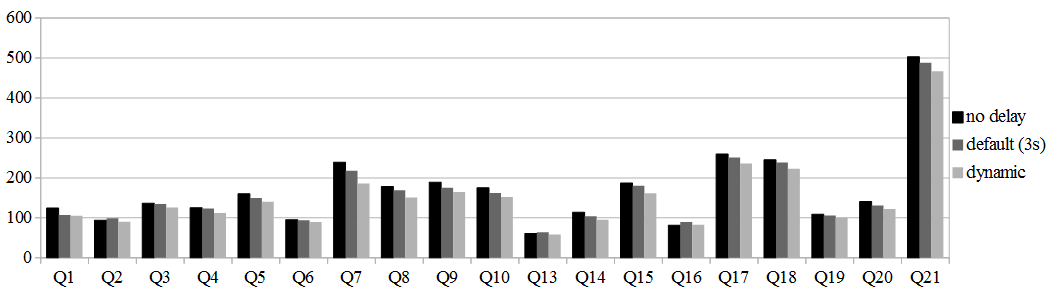
\includegraphics[width=\linewidth]{./TPCH.png}
        \caption{110GB Spark TPC-H Queries - Job Completion Time (s) vs. Delay Type}
        \label{fig:largescale}
    \endminipage \hfill
\end{figure*}

